\section{Drone movement}
%As mentioned before, this project involved the uses of drones, it is necessary to understand some theory of the physics for drones.
The type of multirotor drone that will be used on in this project are a quadcopter, but it is the drone's configuration that will be mostly used \cite{PhysicsofDroneFlight}. The quadcopter is a drone with four rotors, as seen on figure \ref{fig:dronePhysics_1}.
\begin{figure}[H]
    \centering
    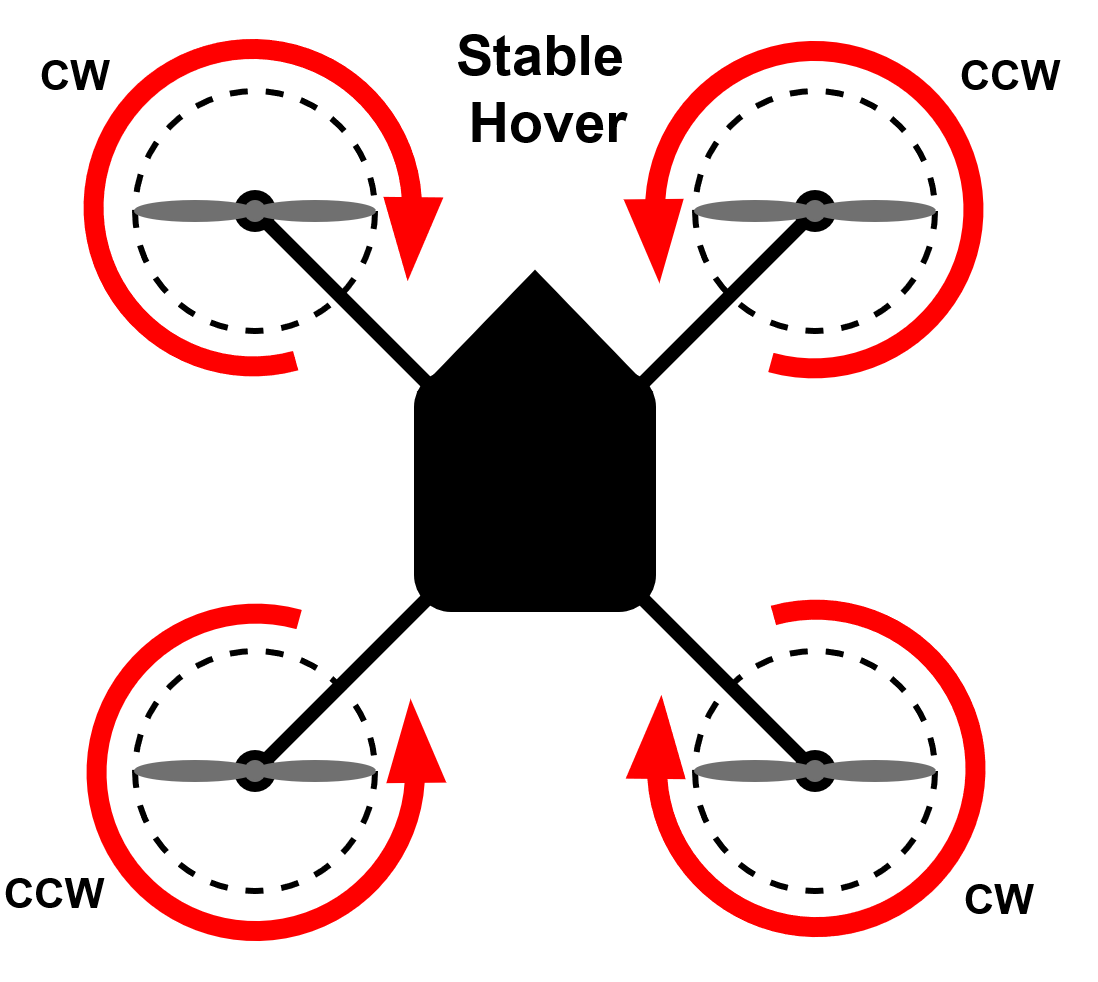
\includegraphics[width=0.3\textwidth]{figures/ch_intro/physics-of-multirotor.png}
    \caption{Illustration of a quadcopter when it is hovering \cite[Redrawn]{PhysicsofDroneFlight}.}
    \label{fig:dronePhysics_1}
\end{figure}
Two of the rotors are configured to rotate clockwise and the other two rotors are counter-clockwise. To control the drone’s movement, the speed of the rotors changes according to the desired action. The different types of movement a drone can do are hovering/altitude control, yaw, roll and pitch.
\newline
\newline
By rotating the rotors, a thrust will be created, see figure \ref{fig:QC_freeBodyDiagram}. This thrust will create a force upward $F_{Thrust}$, if this force are greater than the gravitational pull on the drone $F_g$ and all the rotors rotate has the same speed, it will increase the altitude of the drone. To get the drone to hover in the same position, the thrust must be the same as the gravitational force \cite{PhysicsofDroneFlight}.
\begin{figure}[h]
    \centering
    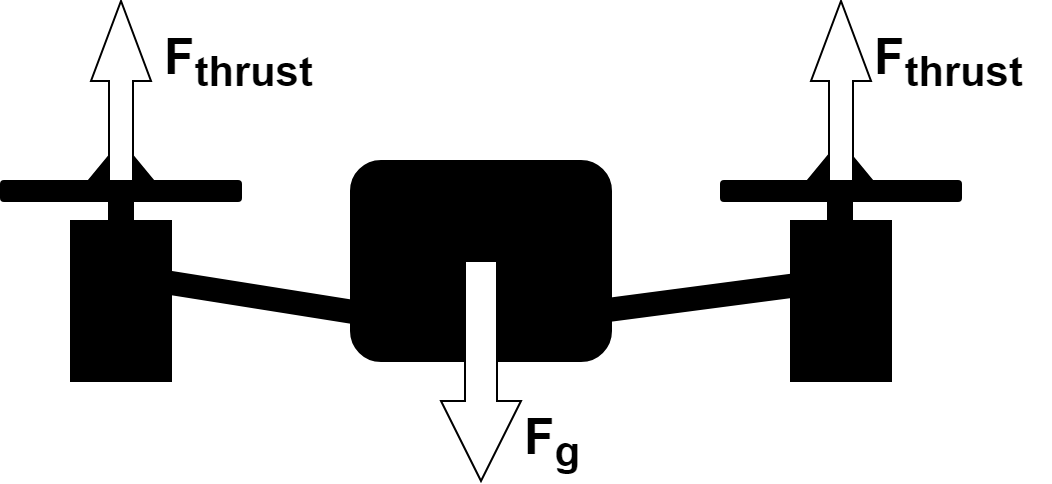
\includegraphics[width=0.45\textwidth]{figures/ch_intro/droen_frit_legeme-diagram.png}
    \caption{Free body diagram of a quadcopter.}
    \label{fig:QC_freeBodyDiagram}
\end{figure}
\newline
\newline
As mentioned previously, one of the movements of the drone is pitching. Pitching the drone tilts it either forward or backwards. By tilting the drone forward, it is possible to get the drone to fly forward. The illustration in figure \ref{fig:dronePhysics_2} shows, the drone can be moved forward by firstly decrease the thrust of the two front rotors and increase the thrust of the two back rotors. This will pitch the drone forward.
\begin{figure}[h]
    \centering
    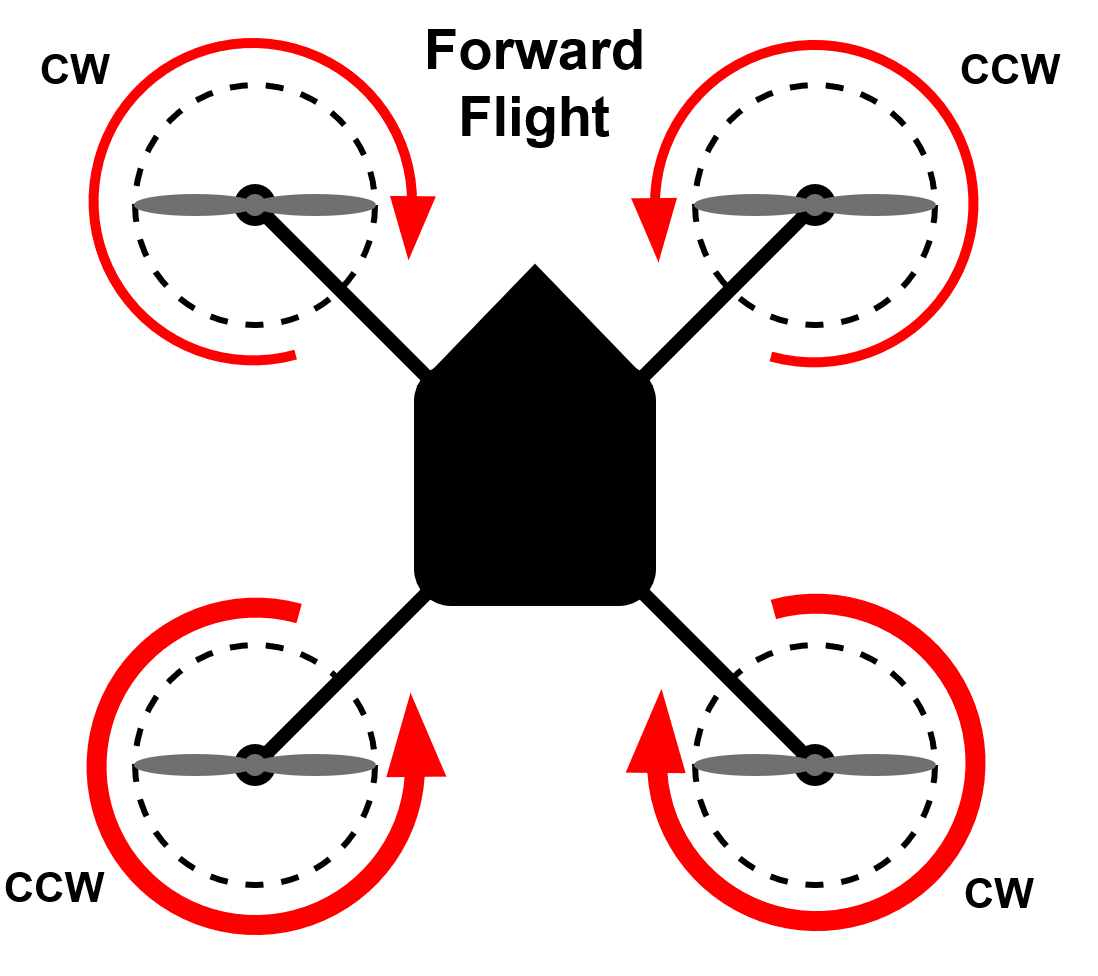
\includegraphics[width=0.3\textwidth]{figures/ch_intro/physics-of-multirotor-2.png}
    \caption{Illustration of a quadcopter when it is flying forward \cite[Redrawn]{PhysicsofDroneFlight}.}
    \label{fig:dronePhysics_2}
\end{figure}
\newline
\newline
After the drone have been pitch forward to a desired angle, all the rotors will then rotate with the same thrust, as when it's hovering but with a slightly higher thrust\cite{PhysicsofDroneFlight}.
\newline
\newline
Sideways movement is equivalent as the forward and backwards movement. The different is that the drone is rolling instead of pitching. To roll/tilt the drone right, the two right rotors decreases its thrust and the left rotors increases its thrust, this can be seen in figure \ref{fig:dronePhysics_3}. After the drone have been tilted right, all the rotors will rotate with the same thrust, to fly right. 
\begin{figure}[h]
    \centering
    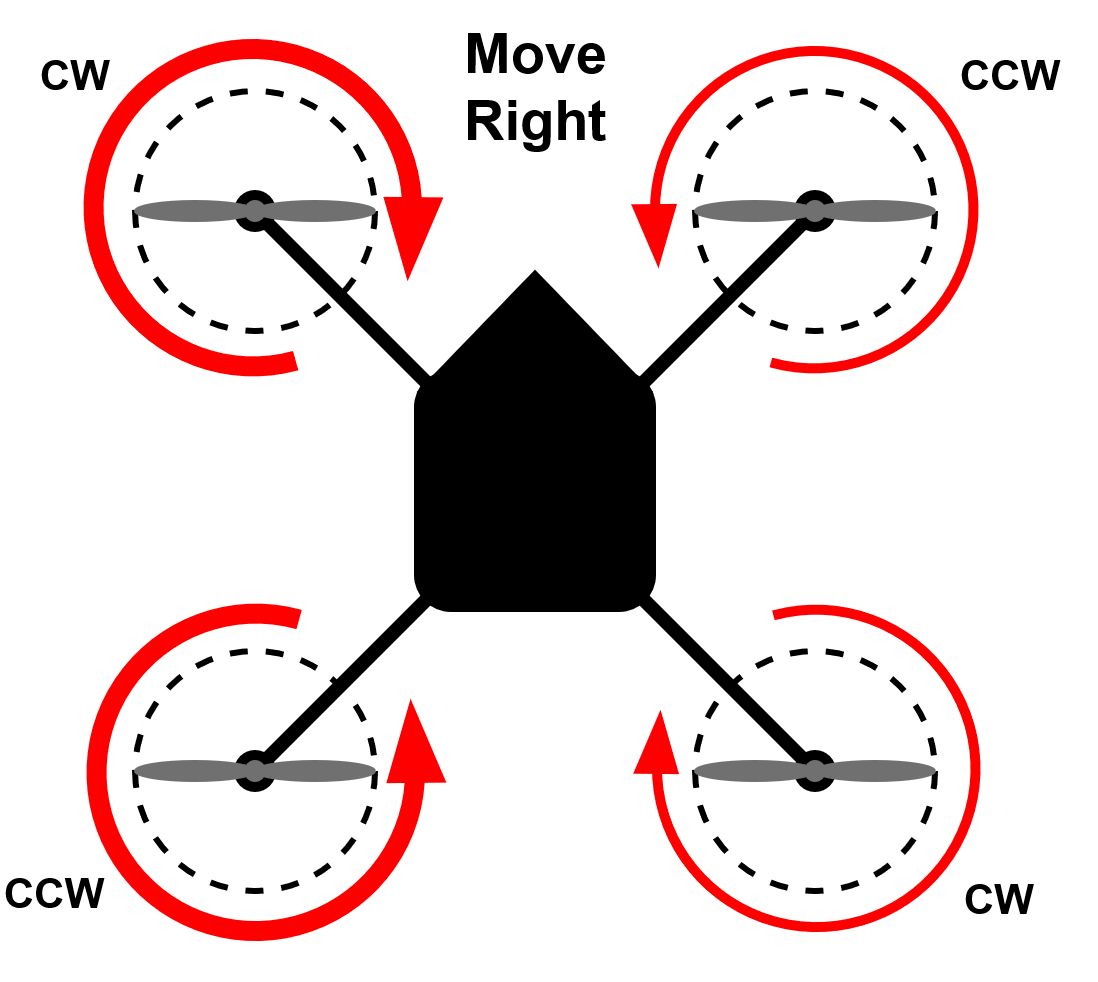
\includegraphics[width=0.3\textwidth]{figures/ch_intro/physics-of-multirotor-3.png}
    \caption{Illustration of a quadcopter when it is flying right \cite[Redrawn]{PhysicsofDroneFlight}.}
    \label{fig:dronePhysics_3}
\end{figure}
\newline
The last type of movement the drone can do is yaw/rotate. To understand how the drone can rotate, it is necessary to look into the rotors. When a rotor rotates it generates a rotational force also known as torque. Because of the torque of a rotor that rotate clockwise, the drone will rotate counter-clockwise. By using a counter-clockwise rotor with the same force, the two opposite torque will cancel each other out\cite{PhysicsofDroneFlight}. This means that the drone does not rotate when tilting. The clockwise rotors are placed opposite of each other, and the same with the counter-clockwise, as it can be seen on figure \ref{fig:dronePhysics_4}.
\newline
\begin{figure}[h]
    \centering
    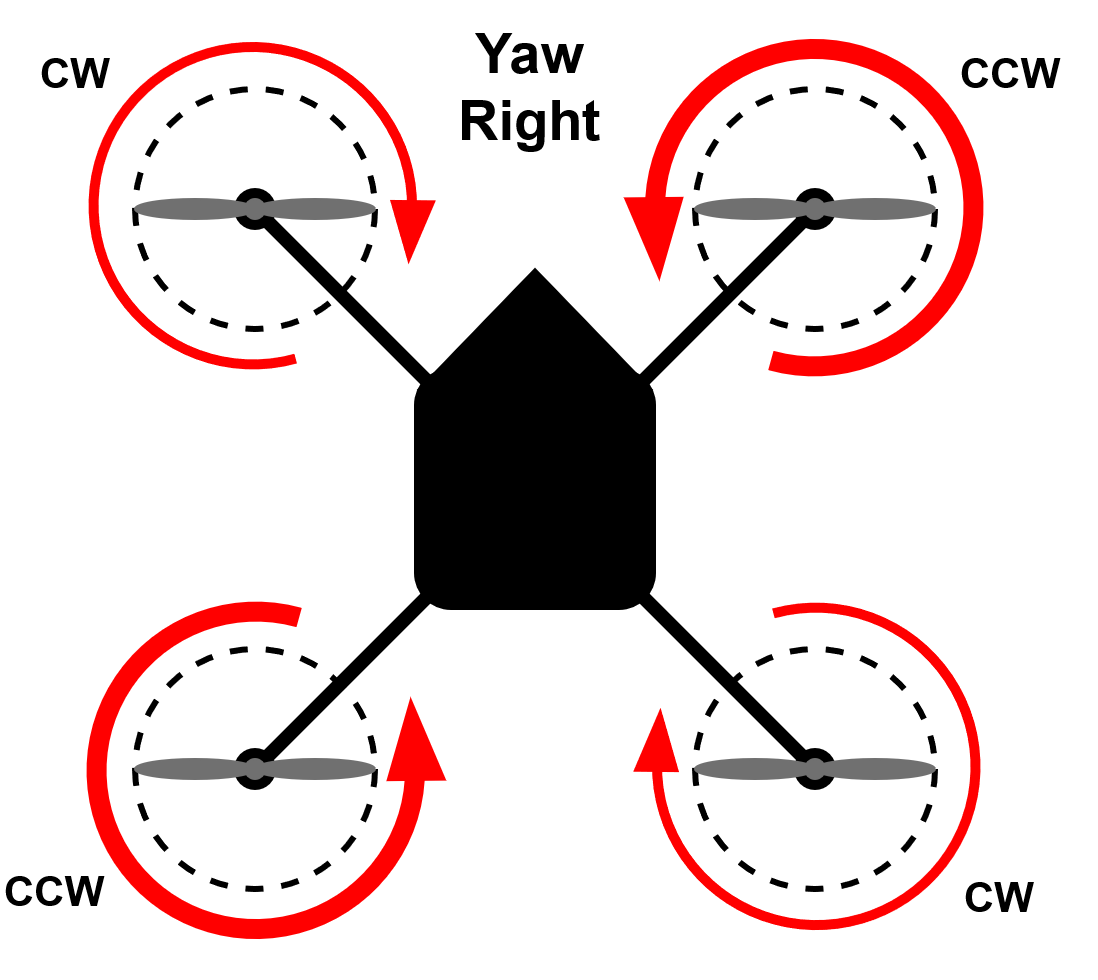
\includegraphics[width=0.3\textwidth]{figures/ch_intro/physics-of-multirotor-4.png}
    \caption{Illustration of a quadcopter when it is rotating right \cite[Redrawn]{PhysicsofDroneFlight}.}
    \label{fig:dronePhysics_4}
\end{figure}
\newline
For the drone to rotate right the two counter-clockwise rotors must increase the thrust, from the hovering state, and the thrust of the clockwise must decrease, which can be seen in figure \ref{fig:dronePhysics_4}. When increasing and decreasing the thrust of the rotors, the total thrust must be the same as in hovering state for it not to lose altitude. 